\section*{Ejercicios}
\begin{enumerate}

\item El receptor trifásico de la figura tiene secuencia de fases
  inversa y tensión de línea 200$\sqrt{3}$ V. Su potencia activa es 12
  kW y el vatímetro 2 ($W_2$) indica 6 kW. Hallar:
  \begin{itemize}
  \item Valor de la impedancia $\overline{Z}$, en forma compleja.
  \item Fasores correspondientes a las intensidades de línea.
  \end{itemize}

\begin{center}
  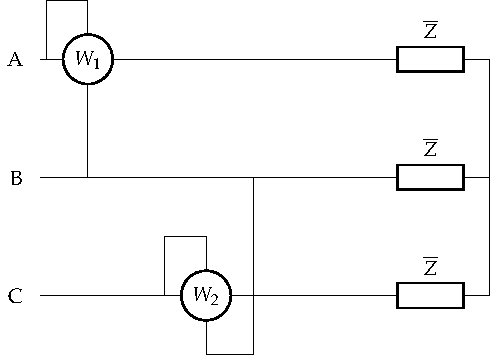
\includegraphics[width=0.5\linewidth]{../figs/ej6_BT3.pdf}
\end{center}

\emph{Sol.:\;
  $\overline{Z}=10\phase{0^\circ}\,\Omega;\;
  \overline{I}_A={20\phase{-90^\circ}\,\mathrm{A}};\;
  \overline{I}_B={20\phase{30^\circ}\,\mathrm{A}};\;
  \overline{I}_C={20\phase{150^\circ}\,\mathrm{A}}$}


\item En el sistema trifásico de la figura, de secuencia de fases
  directa y $f=60$ Hz, el receptor equilibrado disipa una potencia
  total $P_T =51984$ W con un factor de potencia de $0.6$ en
  retraso. Sabiendo que el amperímetro indica 76$\sqrt{3}$ A,
  determinar:
  \begin{itemize}
  \item Lecturas de los vatímetros 1 y 2
  \item Valor de la impedancia $\overline{Z}$ en forma compleja
  \item Capacidad mínima para mejorar el factor de potencia a $0.95$
  \end{itemize}
  \begin{center}
    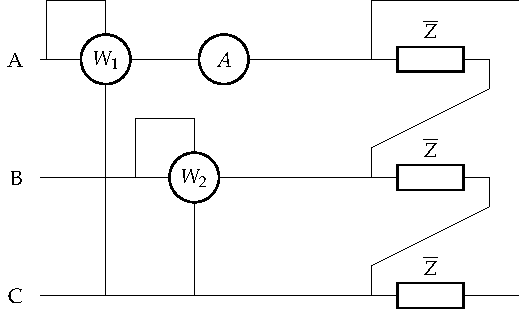
\includegraphics[width=0.54\linewidth]{../figs/ej4_BT3.pdf}
  \end{center}
  \emph{Sol.:\;
    $ W_1=\qty{46000.65}{\watt};\; W_2=\qty{5983.35}{\watt};\;
    \overline{Z}=3+\mathrm{j}\,4\;\Omega;\; C_{\triangle}=\qty{319.8}{\micro\farad}$}

\item En el sistema trifásico de la figura, de secuencia de fases
  inversa y tensión de línea 200$\sqrt{3}$ V, los dos receptores son
  equilibrados, con impedancias
  $\overline{Z}_1 = 6+\mathrm{j}8\;\Omega$ y
  $\overline{Z}_2 = 8+\mathrm{j}6\;\Omega$. Determinar:
  \begin{itemize}
  \item Lecturas de los amperímetros.
  \item Lecturas de los vatímetros y la potencia compleja total.
  \end{itemize}
  \begin{center}
    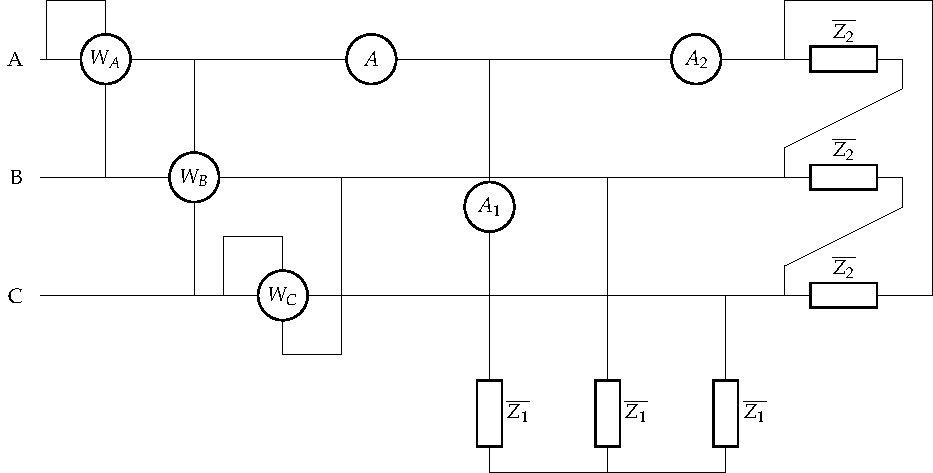
\includegraphics[width=.93\linewidth]{../figs/ej5_BT3.pdf}
  \end{center}

  \emph{Sol.:\;
    $A=\qty{79.40}{\ampere};\;
    A_1=\qty{20}{\ampere};\;
    A_2=\qty{60}{\ampere};\; 
    W_A=\qty{27007.43}{\watt};\;
    W_B=\qty{18013.85}{\watt};\;
    W_C=\qty{8993.58}{\watt};\;
    \overline{S}_T=36+\mathrm{j}\,31.2\,\si{\kilo\voltampere} $}

\item El sistema trifásico de la figura es de 380 V a 50 Hz y
  secuencia de fases inversa. $\overline{Z}$ es un elemento pasivo
  ideal, tal que el factor global de potencia es la unidad. El motor
  es de 1,8 CV, rendimiento 90\% y factor de potencia 0,8. Determinar:
  \begin{itemize}
  \item Impedancia $\overline{Z}$ en forma compleja.
  \item Intensidad en el motor.
  \item Fasores intensidad de línea.
  \item Lectura de los aparatos de medida: V, A, W$_1$, W$_2$ y W$_3$.
  \end{itemize}
  \begin{center}
    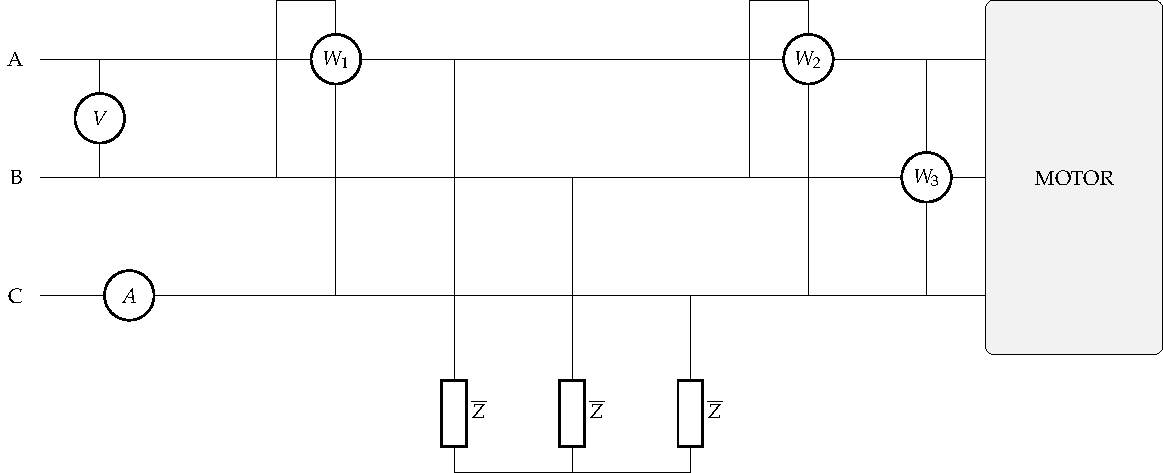
\includegraphics[width=\linewidth]{../figs/ej7_BT3.pdf}
  \end{center}

  \emph{Sol.:\;
    $\overline{Z}={-\mathrm{j}\,129.76}\;\Omega/\mathrm{fase};\;
    I_M=\qty{2.83}{\ampere};\;
    \overline{I}_A={2.27\phase{-90^\circ}\,\si{\ampere}};\;
    \overline{I}_B={2.27\phase{30^\circ}\,\si{\ampere}};\;
    \overline{I}_C={2.27\phase{150^\circ}\,\si{\ampere}};\; 
    \\
    W_1=0;\;
    W_2=\qty{-645.24}{\watt};\; 
    W_3=\qty{645.24}{\watt}$}

\item  Una plantación agrícola emplea dos bombas sumergibles para extraer
 agua de un pozo y transportarla a través de un sistema de riego por
 goteo. Estas dos bombas están alimentadas a \SI{400}{\volt} por una
 línea trifásica en secuencia de fases directa y frecuencia
 $\SI{50}{\hertz}$. Una de las bombas funciona con un motor trifásico
 de $\SI{30}{\kilo\watt}$ y factor de potencia de $0.78$. La otra bomba
 trabaja con un motor de $\SI{7.5}{\kilo\watt}$ y factor de potencia
 de $0.67$.  La línea que alimenta estas dos bombas es resistiva, con
 resistividad $\rho = \SI{0.017}{\ohm\milli\meter\squared\per\meter}$,
 longitud de \SI{300}{m} y una sección de
 \SI{35}{\milli\meter\squared}.
 
 \begin{enumerate}
 \item Calcula el triángulo de potencias (potencia activa, reactiva, y
   aparente) de cada carga, y total de las cargas (a la salida de la
   línea).
 \item Calcula el valor eficaz de la corriente de línea de
   cada carga y de la corriente total.
 \item Determina la lectura de los siguientes aparatos de medida
   conectados a la entrada de las cargas:
   \begin{itemize}
   \item Un vatímetro en la fase A, midiendo tensión entre las fases A
     y C.
   \item Un vatímetro en la fase B, midiendo tensión entre las fases B
     y C.
   \item Un vatímetro en la fase C, midiendo tensión entre las fases B
     y A.
   \end{itemize}
 \item Calcula el triángulo de potencias a la entrada de la línea.
 \item Calcula el valor eficaz de la tensión a la entrada de la línea.
 \item Calcula los condensadores que se deben conectar a la salida de
   la línea para mejorar el factor de potencia del sistema hasta la
   unidad. Indica modo de conexión más eficiente.
 \end{enumerate}

Una vez conectados los condensadores del último apartado:
\begin{enumerate}[resume]
\item Calcula el valor eficaz de la corriente de línea total.
\item Calcula el triángulo de potencias a la entrada de la línea.
\item Calcule el valor eficaz de la tensión a la entrada de la línea.
\item Determina la lectura de los vatímetros descritos anteriormente.
\end{enumerate}

  \emph{Sol.:\;
    $P_1 = \SI{30}{\kilo\watt};\; 
    Q_1 = \qty{24.06}{\kilo\voltampere_r};\; 
    S_1 = \SI{38.46}{\kilo\voltampere};\;
    P_2 = \SI{7.5}{\kilo\watt};\; 
    Q_2 = \qty{8.31}{\kilo\voltampere_r};\; 
    S_2 = \SI{11.19}{\kilo\voltampere}; \;
    P_T = \SI{37.5}{\kilo\watt};\; 
    Q_T = \qty{32.37}{\kilo\voltampere_r};\; S_T = \SI{49.54}{\kilo\voltampere};\; 
    I_1 = \qty{55.51}{\ampere};\; 
    I_2 = \qty{16.15}{\ampere};\; 
    I_T= \qty{71.5}{\ampere};\; 
    W_{A,AC} = \SI{28.09}{\kilo\watt};\;
    W_{B,BC} = \SI{9.41}{\kilo\watt};\;
    W_{C, BA} = \SI{-18.66}{\kilo\watt};\;
    P_g = \SI{39.73}{\kilo\watt};\; 
    Q_g = \qty{32.33}{\kilo\voltampere_r};\; 
    S_g = \SI{51.22}{\kilo\voltampere};\; 
    U_g = \qty{413.64}{\volt};\; 
    C_{\triangle} = \qty{214.4}{\micro\farad}/\mathrm{fase};\;
    I_T' = \qty{54.13}{\ampere};\; 
    P_g' = \SI{38.78}{\kilo\watt};\; 
    Q_g' = \qty{0}{\voltampere_r};\; 
    S_g' = \SI{38.78}{\kilo\voltampere};\; 
    U'_g = \qty{413.63}{\volt};\;
    W_{A,AC}' = \SI{18.75}{\kilo\watt};\;
    W_{B,BC}' = \SI{18.75}{\kilo\watt};\; 
    W'_{C,BA} = \SI{0}{\kilo\watt}$ }

 
\item El circuito de la figura es de secuencia de fases directa y 50
  Hz. Determinar:
  \begin{enumerate}
  \item Potencias activas y reactivas totales.
  \item Capacidad mínima de los condensadores a instalar para mejorar
    el factor de potencia total hasta la unidad.
  \item Intensidades de línea, en forma fasorial, una vez mejorado el
    factor de potencia.
  \end{enumerate}
  \begin{minipage}{0.4\linewidth}

    \vspace{-25mm}
    Datos:
    \begin{align*}
      \overline{Z}_1 &= {100\phase{\ang{60}}}\,\unit{\ohm}\\
      W_1 &= \SI{300}{\watt}\\
      W_2 &= \SI{300}{\watt}\\
      V &= {200\sqrt{3}}\,\unit{\volt}
    \end{align*}
  \end{minipage}
  \begin{minipage}{0.6\linewidth}
    \begin{center}
      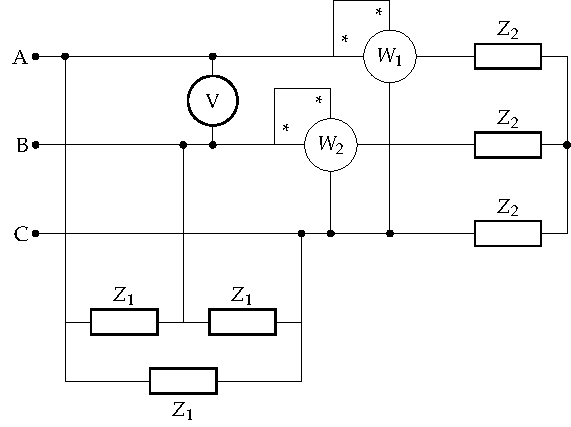
\includegraphics[width=.97\linewidth]{../figs/ZyZt}
    \end{center}
  \end{minipage}
  
  \emph{Sol.:\;
  $P_T = \qty{2400}{\watt};\; 
  Q_T =1800\sqrt{3}\,\si{\voltampere_r};\; 
  C=\qty{27.57}{\micro\farad}/\mathrm{fase};\;
  \overline{I}_A = {4\phase{{90^\circ}}}\,\si{\ampere};\;
  \overline{I}_B = {4\phase{{-30^\circ}}}\,\si{\ampere};\;
  \overline{I}_C = {4\phase{{-150^\circ}}}\,\si{\ampere}$}

  
\item En la figura dos vatímetros miden una carga trifásica inductiva
  equilibrada alimentada a una tensión $U = \SI{400}{\volt}$. El
  vatímetro $W_B$ indica una lectura de \SI{11320}{\watt}, y el
  vatímetro $W_C$ indica una lectura de \SI{1815}{\watt}. A partir de
  esta información se pide:

  \begin{enumerate}
  \item Determinar la secuencia de fases del sistema.
  \item Triángulo de potencias de la carga.
  \item Impedancia equivalente de la carga en estrella y en triángulo.
  \item Tensión de alimentación a la entrada de la línea $U_1$
    sabiendo que la línea de alimentación es resistiva pura con valor
    $R = \SI{0.1}{\ohm}$.
  \item Capacidad de los condensadores que se deben conectar en bornes
    de la carga para conseguir mejorar su factor de potencia a la
    unidad. Determinar las nuevas lecturas de los vatímetros $W_B$ y
    $W_c$.
  \end{enumerate}

\begin{center}
  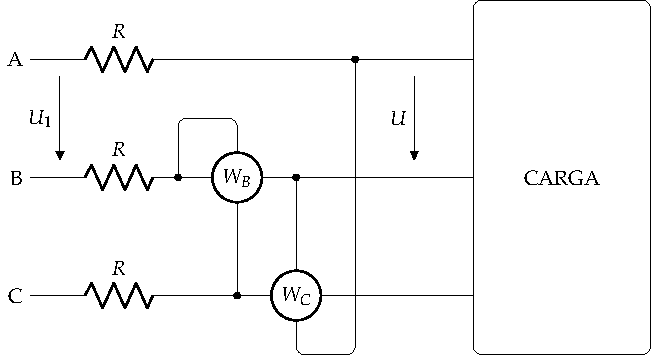
\includegraphics[width=0.64\linewidth]{../figs//BT3_10.pdf}
\end{center}

\emph{Sol.:\; $\mathrm{SFI}$;\; $ P = \qty{20825}{\watt}$;\;
  $Q = \qty{3143.7}{VA}_r$;\;
  $\overline{S} = 21060.9\phase{\ang{8.58}}\,\unit{VA}$;\;
  $\overline{Z}_{\triangle} = {22.8\phase{\ang{8.58}}}\,\unit{\ohm}$;\;
  $U_1 = \SI{405.21}{\volt}$;\; $C = \SI{20.85}{\micro\farad}$ }

\item Del circuito de la figura se sabe que tiene una secuencia de
  fases directa ABC. El amperímetro indica $\SI{5}{\ampere}$, el
  voltímetro $\SI{400}{\volt}$, y los vatímetros A y C muestran una
  lectura idéntica. Se pide:

  \begin{enumerate}
  \item Valor de la impedancia Z en forma compleja.
  \item Expresión fasorial de todas las intensidades del circuito.
  \item Lecturas de los vatímetros A y C.
  \end{enumerate}

Dato: $\; \overline{Z}_L = \SI[parse-numbers = false]{1 + j}{\ohm}$
\begin{center}
  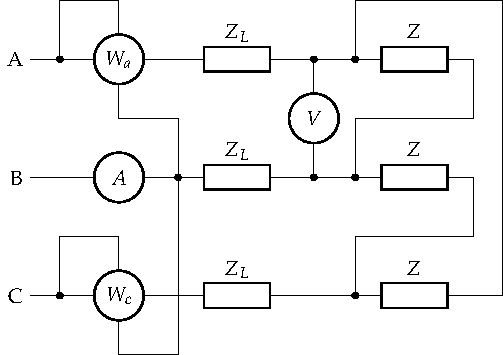
\includegraphics[width = 0.5\textwidth]{../figs/BT3_12}
\end{center}


\emph{Sol.:\; $ Z = \SI[parse-numbers=false]{80\sqrt{3}}{\ohm}$;\;
  $ \overline{I}_A = {5\phase{91.24^\circ}}\,\unit{\ampere}$;\;
  $ \overline{I}_B = {5\phase{-28.75^\circ}}\,\unit{\ampere}$;\;
  $ \overline{I}_C = {5\phase{-148.75^\circ}}\,\unit{\ampere}$;\;
  $ W_a = W_c = \SI{1761.04}{\watt}$}

\item En el circuito de la figura se debe determinar:

\begin{enumerate}
\item Lectura del vatímetro $W_c$.
\item Lectura del amperímetro.
\item Factor de potencia total de las cargas (en retraso o adelanto).
\item Lectura de los vatímetros $W_a$ y $W_b$.
\item Lectura del voltímetro.
\item Valor de los condensadores conectados en $A_1B_1C_1$ para que el
  f.d.p. en ese punto sea la unidad.
\item Lecturas de los cinco aparatos de medida tras el apartado
  anterior.
\end{enumerate}

Datos:
\begin{itemize}
\item Secuencia de fases directa, $f = \SI{50}{\hertz}$, ($A_1B_1C_1$)
  $U_1 = \SI{420}{\volt}$.
\item $Z_1$: motor de 10 CV, con $\eta = 0.83$, y f.d.p. de $0.9$.
\item $Z_2$: conjunto de iluminación fluorescente, con
  $P = \SI{2400}{\watt}$, y f.d.p. de $0.85$.
\item $R_L = \SI{1}{\ohm}$.
\end{itemize}

\begin{center}
  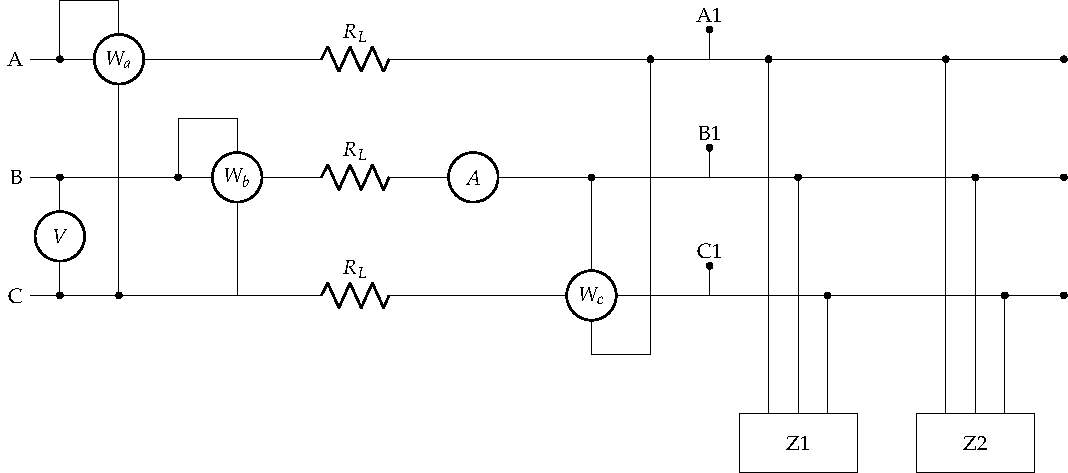
\includegraphics[width=0.95\textwidth]{../figs/BT3_11.pdf}
\end{center}

\emph{Sol.:\; $ W_c = \qty{-3338.3}{\watt}$;\;
  $ A = \SI{17.41}{\ampere}$;\; $ fdp = 0.89$;\;
  $ W_A = \SI{7757.6}{\watt}$;\; $ W_B = \SI{4419.27}{\watt}$;\;
  $ U' = \SI{447.02}{\volt}$;\; $ C = \SI{34.78}{\micro\farad}$}

\item Una línea ideal trifásica de 4 hilos alimenta a dos cargas a una
  tensión de $\SI{400}{\volt}$ en secuencia de fases inversa (SFI) y
  frecuencia $\SI{50}{\hertz}$.

  Las cargas tienen las siguientes características:

  \begin{itemize}
  \item Un motor trifásico de $\SI{70}{\kilo\watt}$ y f.d.p. de $0.8$.
  \item Un conjunto equilibrado de 90 lámparas fluorescentes. Las
    características de cada lámpara son: potencia de $\SI{12}{\watt}$,
    f.d.p. de $0.7$ en retraso, tensión $\SI{230}{\volt}$.
  \end{itemize}

  Con esta información se pide:

  \begin{enumerate}
  \item Conectar adecuadamente los siguientes aparatos de medida antes
    de las cargas:
    \begin{itemize}
    \item Un voltímetro que mida la tensión de línea (etiquetado como
      $V_L$) y otro voltímetro que mida la tensión de fase (etiquetado
      como $V_F$).
    \item Un vatímetro que permita calcular la potencia reactiva total
      del sistema (etiquetado como $W_r$).
    \item Dos vatímetros que, de forma conjunta, permitan calcular la
      potencia activa total del sistema (etiquetados como $W_X$ y
      $W_Y$).
    \end{itemize}
  \item Calcular el valor eficaz de la corriente de línea total.
  \item Calcular la lectura de cada uno de los aparatos de medida del
    primer apartado.
  \item Calcular los condensadores necesarios para mejorar el factor
    de potencia hasta $0.9$, indicando cómo se deben conectar.
  \item Una vez conectados los condensadores del anterior apartado,
    determinar la corriente de línea y la lectura de todos los
    aparatos de medida del apartado 2.
  \end{enumerate}

  \emph{Sol.:\; $I = \qty{128.5}{\ampere}$;\; $V_L = \qty{400}{\volt}$;\;
    $V_F = \qty{230.9}{\volt}$;\; $W_r = \qty{30947}{\watt}$;\;
    $W_X = \qty{20666.5}{\watt}$;\; $W_Y = \qty{51013.5}{\watt}$;\;
    $C=\SI{127.2}{\micro\farad}$;\; $I' = \qty{114}{\ampere}$;\;
    $W'_X = \SI{25602.2}{W}$;\; $W'_Y = \SI{45477.8}{W}$;\;
    $W'_R = \SI{19875.6}{W}$}

\item

  En el sistema de la figura de secuencia de fases directa y
  frecuencia $f=\qty{60}{\hertz}$, se dispone de un receptor
  equilibrado con una potencia total $P_T=\qty{51984}{\watt}$ y factor
  de potencia de $0.6$ en retraso. Sabiendo que el amperímetro marca
  $\qty[parse-numbers=false]{76\sqrt{3}}{\ampere}$, determinar:
  \begin{enumerate}
  \item Medida de los vatímetros 1 y 2.
  \item Valor de la impedancia $\overline{Z}$ en forma
    módulo-argumento.
  \item Valor de la capacidad mínima para mejorar el factor de
    potencia a $0.95$ en retraso.
  \item Valor de la impedancia equivalente en estrella.
  \end{enumerate}
  \begin{center}
    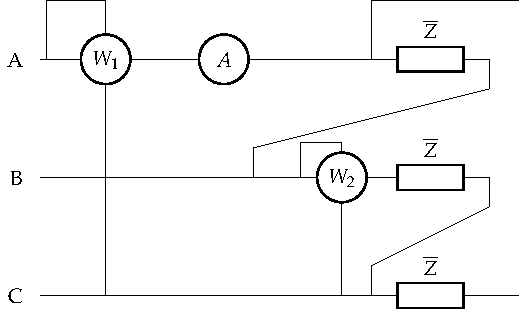
\includegraphics[scale=0.9]{../figs/dosvat_triangulo.pdf}
  \end{center}
  
  \emph{Sol.:\; $W_1 = \qty{46001}{\watt}$;\; $W_2=\qty{17328}{\watt}$;\;
    $\overline{Z} = {5\phase{\ang{53.13}}}\,\unit{\ohm}$}

  
\item Un sistema trifásico a cuatro hilos de $\qty{200}{\volt}$, $\qty{50}{\hertz}$ y secuencia de fases directa está constituido por un motor a cuatro hilos de $\qty{3200}{\watt}$ de potencia y factor de potencia de $0.9$, y un triángulo de impedancias  $20\phase{\ang{30}}\,\unit{\ohm}$. Con esta información, se debe determinar:

\begin{enumerate}
\item Impedancia equivalente del motor.
\item Impedancia equivalente de todo el sistema.
\end{enumerate}

\emph{Sol:\;
  $\overline{Z}_{m\wye} = 11.25\phase{\ang{25.84}}\,\unit{\ohm}$;\;
  $\overline{Z}_{\wye} = 4.19\phase{\ang{28.45}}\,\unit{\ohm}$
}

\item En el circuito de la figura la tensión es $275\sqrt{3}\,\unit{\volt}$. Los motores 1 y 2 tienen factores de potencia $0.96$ y $0.8$, respectivamente. El vatímetro $W_a$ da una lectura de $2420\sqrt{3}\,\unit{\watt}$. Al medir las intensidades de los motores se comprueba que son iguales en ambos. Con esta información se debe determinar:

\begin{enumerate}
\item Secuencia de fases del sistema.
\item Lectura del vatímetro $W_b$.
\item Impedancias de cada uno de los motores e impedancia equivalente del conjunto.
\end{enumerate}

\begin{center}
  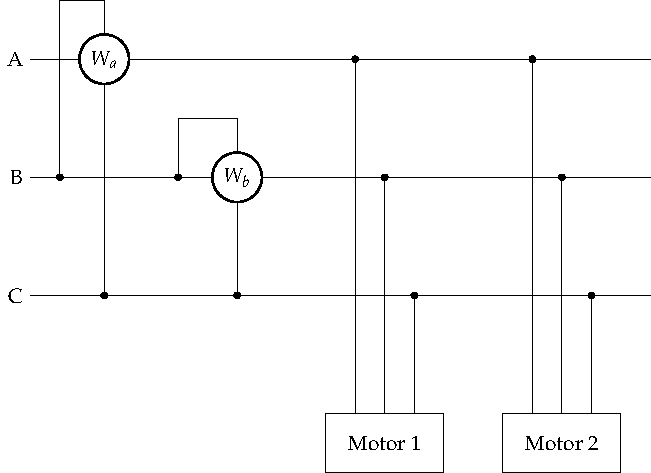
\includegraphics[height=0.27\textheight]{../figs/BT3_13}
\end{center}

\emph{Sol.:\;
  $\mathrm{SFD}$;\;
  $W_b = \qty{5164.2}{\watt}$;\;
  $\overline{Z}_{1\wye} = 27.5\phase{\ang{16.26}}\,\unit{\ohm}$;\;
  $\overline{Z}_{2\wye} = 27.5\phase{\ang{36.87}}\,\unit{\ohm}$;\;
  $\overline{Z}_{\wye} = 13.97\phase{\ang{26.56}}\,\unit{\ohm}$
  }

\end{enumerate}

%%% Local Variables:
%%% mode: latex
%%% TeX-master: "enunciados_ejercicios_TC"
%%% ispell-local-dictionary: "castellano"
%%% End:
